\documentclass[12pt,a4paper]{article}
\usepackage[utf8]{inputenc}
\usepackage[T1]{fontenc}
\usepackage[english]{babel}
\usepackage{lmodern}
\usepackage{csquotes}
\usepackage{amsmath}
\usepackage{amssymb}
\usepackage{physics}
\usepackage{geometry}
\usepackage{tocloft}
\usepackage{xcolor}
\usepackage{graphicx,tikz,pgfplots}
\pgfplotsset{compat=1.18}
\usepackage{booktabs}
\usepackage{siunitx}
\usepackage{amsthm}
\usepackage[colorlinks=true, linkcolor=blue, citecolor=blue, urlcolor=blue]{hyperref}
\usepackage{cleveref}

\geometry{a4paper, margin=2cm}

\renewcommand{\cftsecfont}{\color{blue}}
\renewcommand{\cftsubsecfont}{\color{blue}}
\renewcommand{\cftsecpagefont}{\color{blue}}
\renewcommand{\cftsubsecpagefont}{\color{blue}}
\setlength{\cftsecindent}{1cm}
\setlength{\cftsubsecindent}{2cm}

\newcommand{\Tfield}{T(x)}

\newtheorem{theorem}{Theorem}[section]
\newtheorem{proposition}[theorem]{Proposition}

\title{The Necessity of Extending Standard Quantum Mechanics and Quantum Field Theory}
\author{Johann Pascher}
\date{March 27, 2025}

\begin{document}
	
	\maketitle
	
	\begin{abstract}
		This work examines the conceptual limitations of standard quantum mechanics (QM) and quantum field theory (QFT), proposing the time-mass duality with an intrinsic time field as an extension. By introducing \(\Tfield = \hbar/mc^2\), a link between time and mass is established, overcoming the QM-QFT duality and providing a deterministic framework. The theory is supported by experimental predictions and cosmological implications.
	\end{abstract}
	
	\tableofcontents
	\newpage
	
	\section{Introduction: Conceptual Limits of Established Theories}
	QM and QFT face limits, particularly in integrating with General Relativity (GR) and understanding time and mass. The time-mass duality offers a new approach \cite{pascher_wesentl_2025}.
	
	\subsection{Inherent Duality between QM and QFT}
	\begin{itemize}
		\item QM: Particle perspective \cite{schrodinger}.
		\item QFT: Field-based view.
	\end{itemize}
	
	\subsection{Overinterpretation Due to Incomplete Theoretical Foundations}
	\begin{itemize}
		\item Measurement problem \cite{einstein2}.
		\item Nonlocality \cite{bell}.
	\end{itemize}
	
	\section{Asymmetric Treatment of Time and Space}
	\subsection{Time as Parameter vs. Space as Operator}
	\begin{equation}
		i\hbar \frac{\partial}{\partial t}\Psi(x,t) = \hat{H}\Psi(x,t)
	\end{equation}
	
	\section{Static Treatment of Mass}
	\subsection{Mass as an Invariable Parameter}
	\begin{equation}
		\hat{H} = \frac{\hat{p}^2}{2m} + V(\hat{x})
	\end{equation}
	
	\section{The Concept of Intrinsic Time}
	\begin{theorem}[Intrinsic Time]
		\begin{equation}
			\Tfield = \frac{\hbar}{mc^2}
		\end{equation}
	\end{theorem}
	
	\section{Time-Mass Duality: A New Theoretical Framework}
	\subsection{Complementary Models}
	\begin{itemize}
		\item Standard Model: Constant mass.
		\item T0 Model: Absolute time.
	\end{itemize}
	
	\subsection{Reformulation of the Schrödinger Equation}
	\begin{equation}
		i\hbar \frac{\partial}{\partial (t/\Tfield)}\Psi = \hat{H}\Psi
	\end{equation}
	
	\section{Consequences for Fundamental Phenomena}
	\subsection{Quantum Coherence and Decoherence}
	\begin{equation}
		\Gamma_{\text{dec}} = \Gamma_0 \cdot \frac{mc^2}{\hbar}
	\end{equation}
	
	\begin{figure}[h]
		\centering
		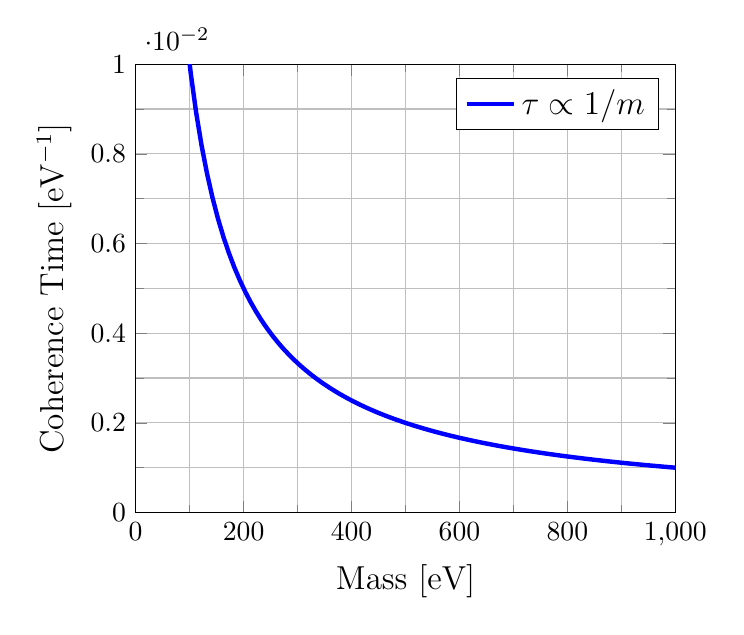
\begin{tikzpicture}
			\begin{axis}[
				xlabel={Mass [eV]},
				ylabel={Coherence Time [eV\(^{-1}\)]},
				xlabel style={font=\large},
				ylabel style={font=\large},
				tick label style={font=\normalsize},
				xmin=0, xmax=1000,
				ymin=0, ymax=0.01,
				legend pos=north east,
				legend style={font=\large},
				grid=both,
				minor tick num=1
				]
				\addplot[blue, ultra thick, domain=1:1000, samples=100] {1/x};
				\legend{\(\tau \propto 1/m\)}
			\end{axis}
		\end{tikzpicture}
		\caption{Mass-dependent coherence time in the T0 model.}
	\end{figure}
	
	\section{Variable Mass as a Hidden Variable}
	\subsection{Modified Quantum Dynamics}
	\begin{equation}
		i\hbar \frac{\partial}{\partial t}\Psi(x,t) = \hat{H}(m(t))\Psi(x,t)
	\end{equation}
	
	\section{Cosmological Implications}
	\begin{itemize}
		\item Redshift: \(1 + z = e^{\alpha r}\) \cite{pascher_wesentl_2025}.
		\item Gravitational potential: \(\Phi(r) = -\frac{GM}{r} + \kappa r\) \cite{pascher_wesentl_2025}.
	\end{itemize}
	
	\begin{thebibliography}{99}
		\bibitem{pascher_wesentl_2025} Pascher, J. (2025). \textit{Essential Mathematical Formalisms of the Time-Mass Duality Theory with Lagrangian Densities}.
		\bibitem{einstein} Einstein, A. (1905). \textit{Does the Inertia of a Body Depend Upon Its Energy Content?}. Annalen der Physik, 323(13), 639-641.
		\bibitem{planck} Planck, M. (1901). \textit{On the Law of Distribution of Energy in the Normal Spectrum}. Annalen der Physik, 309(3), 553-563.
		\bibitem{schrodinger} Schrödinger, E. (1926). \textit{An Undulatory Theory of the Mechanics of Atoms and Molecules}. Physical Review, 28(6), 1049-1070.
		\bibitem{bell} Bell, J. S. (1964). \textit{On the Einstein Podolsky Rosen Paradox}. Physics, 1(3), 195-200.
		\bibitem{einstein2} Einstein, A., Podolsky, B., Rosen, N. (1935). \textit{Can Quantum-Mechanical Description of Physical Reality Be Considered Complete?}. Physical Review, 47(10), 777-780.
	\end{thebibliography}
	
\end{document}